% ═══════════════════════════════════════════════════════════════════════
\section{Un internaute qui navigue au hasard}
% ═══════════════════════════════════════════════════════════════════════

\begin{frame}{Quelles pages sont les plus importantes ?}
  \begin{columns}[c]
    \begin{column}{0.52\textwidth}
      \small
      \begin{itemize}
        \item Une requête : des millions de pages contiennent les mots
          cherchés. Dans quel ordre les présenter ?
        \item Brin et Page (Stanford, fin des années 1990) : imaginons un
          internaute qui clique au hasard sur les liens, et mesurons la
          proportion du temps qu'il passe sur chaque page.
        \item Une page souvent visitée est une page importante : c'est
          l'idée de PageRank, et de Google.
      \end{itemize}
    \end{column}
    \begin{column}{0.46\textwidth}
      \FigBox[0.5\textheight]{%
        \begin{tikzpicture}[scale=1.15]
          \node[pageweb] (p1) at (0,2.4) {$1$};
          \node[pageweb] (p5) at (3.2,2.4) {$5$};
          \node[pageweb] (p2) at (0,0) {$2$};
          \node[pageweb] (p3) at (2.2,0) {$3$};
          \node[pageweb] (p4) at (4.4,0) {$4$};
          \draw[lien2] (p1) -- (p2);
          \draw[lien2] (p2) -- (p3);
          \draw[lien2] (p3) -- (p4);
          \draw[lien] (p3) -- (p5);
          \draw[lien] (p4) -- (p5);
          \draw[lien] (p5) -- (p1);
          \draw[lien] (p5) -- (p2);
        \end{tikzpicture}}
      \scriptsize Figure 4.1 --- Un mini-web de cinq pages. La page $2$
      reçoit quatre liens, la page $1$ deux : où l'internaute
      passera-t-il le plus de temps ?
    \end{column}
  \end{columns}
\end{frame}

\begin{frame}{Une chaîne de Markov}
  \small Le déplacement de l'internaute est une chaîne de Markov : un
  phénomène aléatoire qui évolue par étapes, dont l'état à l'étape $n+1$
  ne dépend que de l'état à l'étape $n$, et non de tout le passé.
  \vspace{4pt}

  Usages : météorologie, démographie, génétique, finance, reconnaissance
  de la parole, génération de texte.
  \vspace{6pt}

  Le chemin du chapitre :
  \begin{enumerate}
    \item rappels de probabilités ;
    \item deux modèles : la météo à deux états, la migration
      ville--banlieue--campagne ;
    \item chaînes de Markov, matrices de transition ;
    \item le long terme : un vecteur propre de valeur propre $1$ ;
    \item PageRank, avec les difficultés du Web réel ;
    \item le calcul par la méthode des puissances --- et le retour du
      théorème de Banach.
  \end{enumerate}
\end{frame}

\begin{frame}{Note historique 4.1 --- Andreï Markov (1856--1922)}
  \footnotesize
  \begin{columns}[T]
    \begin{column}{0.25\textwidth}
      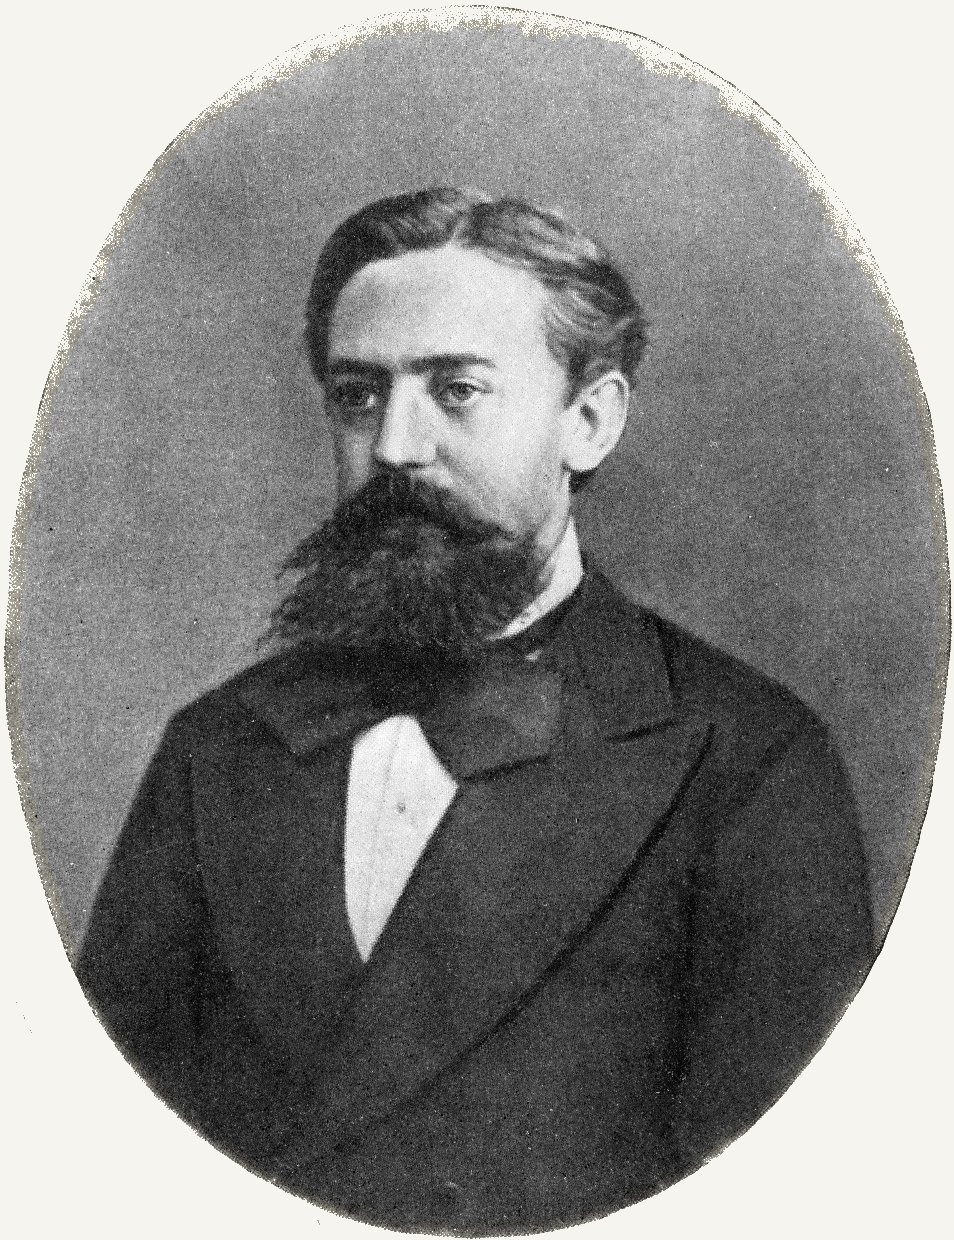
\includegraphics[width=\linewidth]{andrei-markov.jpg}\\
      {\scriptsize\color{gray}Vers 1875. Domaine public,
      Wikimedia Commons.}
    \end{column}
    \begin{column}{0.72\textwidth}
      \begin{itemize}
        \item Né à Riazan ; enfant de santé fragile, il se déplace avec
          des béquilles jusqu'à une dizaine d'années.
        \item Élève de Tchebychev à Saint-Pétersbourg, où il enseigne
          toute sa carrière.
        \item 1906 : ses chaînes, contre Nekrassov, qui soutenait que la
          loi des grands nombres exige l'indépendance (et en tirait des
          conclusions sur le libre arbitre). Markov montre qu'une
          dépendance « au précédent seulement » suffit.
      \end{itemize}
    \end{column}
  \end{columns}
\end{frame}

\begin{frame}{Note historique 4.1 (suite)}
  \small
  \begin{itemize}
    \item Ses chaînes étaient d'abord, pour lui, un contre-exemple
      théorique ; il ne les appliqua qu'une fois à des données réelles
      (note historique 4.2).
    \item Un esprit indépendant : en 1902, il proteste quand l'Académie,
      à la demande du tsar, annule l'élection de Maxime Gorki ; en 1912,
      il demande à être excommunié, par solidarité avec Tolstoï.
    \item En 1913, pendant que l'Empire fête le tricentenaire des
      Romanov, il organise plutôt le bicentenaire de la loi des grands
      nombres (Bernoulli, Ars conjectandi, 1713).
    \item Son fils, Andreï Andreïevitch Markov (1903--1979), sera lui
      aussi mathématicien, spécialiste de logique.
  \end{itemize}
\end{frame}
